\documentclass{article}

\usepackage{amssymb}
\usepackage{amsfonts}
\usepackage{amsmath}
\usepackage[utf8]{inputenc}
\usepackage[T1]{fontenc}

\usepackage[margin=0.5in]{geometry}
\usepackage{hyperref}

\usepackage{graphicx}

\title{Taller 1}
\author{Miguel A. Gomez B.}

\begin{document}
	\maketitle

\paragraph{Plot} The results are too big to be handled by the python graphics library, which is why I only plot those my computer can manage to graph:
\begin{center}
	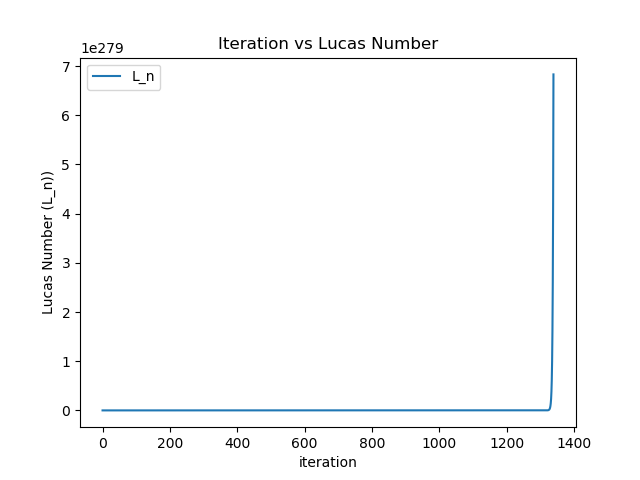
\includegraphics[width=0.8\textwidth]{Plot}
\end{center}

The entire dataset calculated is on the file \textit{values} available at \url{https://github.com/mangel/simulation/blob/master/20202/w1/HW1/values.tar.xz} and is a csv, delimited by '|', the first column is the iteration and the second column is the Lucas number.

\paragraph{Biggest Lucas Number founded}
\paragraph{} Actually is too big to put it here, the size of the file that contains it is almost 5M, it is called \textit{biggest}, and the number was founded at iteration $19800000$\footnote{Actually i let it run for roughly 8 hours}.\\

\paragraph{link} \url{https://github.com/mangel/simulation/blob/master/20202/w1/HW1/biggest}

\end{document}
